\documentclass[10pt,a4paper,oneside,abstracton]{scrartcl}
\usepackage[utf8]{inputenc}
\usepackage[english, ngerman]{babel}

\usepackage{gensymb}
% \usepackage[T1]{fontenc}

\usepackage{amsmath}
\usepackage{amsfonts}
\usepackage{amssymb}
\usepackage{graphicx}
\usepackage{lmodern}
	%\usepackage{kpfonts}
\usepackage{fourier}
\usepackage[left=2cm,right=2cm,top=2cm,bottom=2cm]{geometry}
\usepackage{multicol}
\setcounter{secnumdepth}{4} %Nummerierungstiefe bis Paragraph (4. Ebene)
\usepackage{blindtext}
\usepackage[ 		%Einstellungen für Link
   colorlinks,        % Link ohne Umrandungen in zu wählender Farbe 
   linkcolor=black,   % Farbe interner Verweise 
   filecolor=black,   % Farbe externer Verweise 
   citecolor=black    % Farbe von Zitaten 
]{hyperref}



\newenvironment{Figure}
  {\par\medskip\noindent\minipage{\linewidth}}
  {\endminipage\par\medskip}


\pagestyle{empty}		%Seitenzahl wird nich angezeigt

\begin{document}

\section*{Praktische Auslegung einer elektrischen und thermischen Simulation einer Platine zur Ansteuerung einer Leistungselektronik}
\section*{Christian Schmid}
Hochschule Augsburg, Fakultät für Elektrotechnik, Augsburg, Deutschland, Christian.Schmid1@Hs-Augsburg.de 


\begin{abstract} %kann man auch ueber /subsection machen
\noindent %einrücken verhindern
In dieser Arbeit wird die thermische Auslegung des Leiterbahnquerschnitt einer handelsüblichen gedruckten Leiterplatine(PCB) untersucht. 
Daraus soll bestimmt werden, wie stark sich die Vorgabe aus der Indsutrie mit den von Comsol simulierten Werten unterscheidet. 
Zur Berechnung werden Verfahren aus der Lehre und der Industrie verwendet. 
Es wird eine Daumenregel mit einer Spice Simulation und dem Model vom Comsol verglichen und die Gründe für die 
unterschiedlichen Temperaturen erörtert. 
\end{abstract}

\renewcommand{\abstractname}{Abstract} %aendert name Zusammenfassung in Abstract

\begin{abstract}
\noindent %einrücken verhindern
In this dissertation the thermal dimensioning  of a trace-profile on a  common Printed-Circuit-Board(PCB) is examined.
Industrial standards will be examined and compared with the calculated and simulated results from Comsol.
Standards from education and industries will be used for the calcualtions.  
A rule of thumb, a Spice simulation and a Comsol model will be compared and the discussed regarding different results. 
\end{abstract}


\begin{multicols}{2}
\section{Grundlagen}

\subsection{Wärmefluss}
Es gibt 3 Wärmeausbreitungsmöglichkeiten.  
Durch Konvektion und Strahlung wird die Enerige an die Umluft abgegeben.
Durch Konduktion fließt die Wärme durch die Platine und in das Gehäuse, siehe Abbildung \ref*{l_Waermefluss}.

\begin{Figure}
	% \resizebox{0.1\columnwidth}{!} 
	\includegraphics[width=\textwidth]{Bilder/Wärmestrom.png}
	\captionof{figure}{Wärmefluss auf einer Platine, \cite{Waermefluss}}
	\label{l_Waermefluss}
\end{Figure}

\subsection{Thermische Auslegung}
Elektrische Bauteile werden vom Hersteller im Betriebstemperaturbereich getestet und ausgelegt. 
Bei größerer Betriebstemperatur nimmt die Lebenszeit der Bauteile ab. 
\newline
Besonders gefährdet sind zum Beispiel Elektrolyt Kondensatoren. 
Meist beträgt die maximale Temperatur $ 105 \degree C $ oder weniger. \newline 
Bei Erhöhung der Betriebstemperatur um jeweils $ 10K $ halbiert sich die Lebensdauer der Bauteile \cite{Elko}.
\newline
Ziel sind niedrige Temperaturen durch geringe thermischen Verluste. 
\newline
Die Leiterbahn wird abhängig von der Anwendung unterschiedlich ausgelegt um 
elektrische Verluste durch Selbstinduktion und Widerstand gering zu halten. 
\newline
Eine Versorungsleitung führt einen größeren Strom und benötigt daher einen größeren Leiterbahnquerschnitt als eine Messleitung.
Der Strom geht quadratisch in die Leistungsformel ein, siehe Formel \ref*{Leistung_Strom}. 
\begin{equation}
	P_{elektrisch} = P_{Thermisch} =  I^2 \cdot R_{Leiter} 
	\label{Leistung_Strom}
\end{equation}

\subsection{Leistungselektronik}
% Der Brushless DC Motor ist eine Synchronmaschine. 
% Eine Synchronmaschine braucht 3 zueinander versetzte Phasen mit Spannungen, die einen sinus darstellen.
In der Leistungselektronik wird getaktet an- und abgeschaltet. 
Die Schaltfrequenz ist einige Dekaden größer als die Nutzfrequenz. 
Das System ist träger als die Schaltfrequenz.
Das Verfahren in Abbildung \ref*{Aussteuerung} wird zur Aussteuerungvon Motoren verwendet.
\begin{Figure}
	% \resizebox{0.1\columnwidth}{!} 
	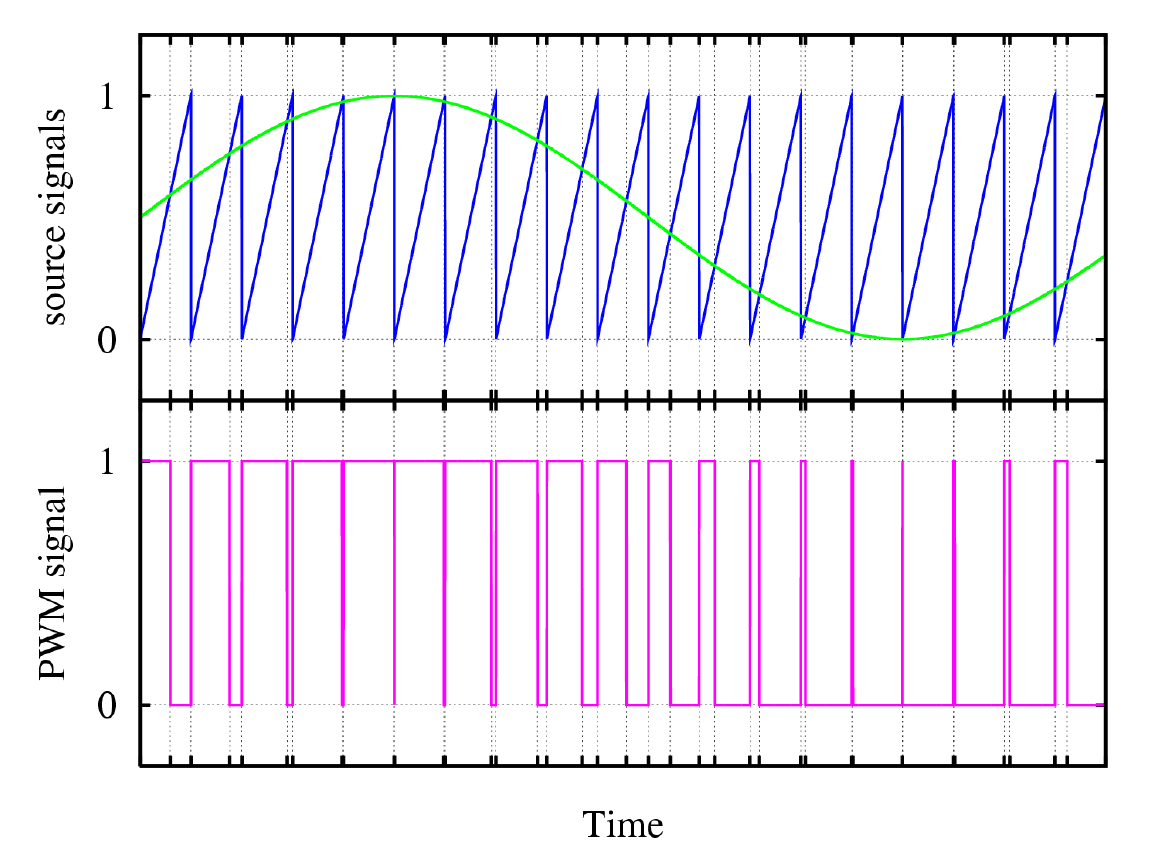
\includegraphics[width=\textwidth]{Bilder/BLDC_Aussteuerung.png}
	\captionof{figure}{Aussteuerung einer Phase eines Motors, \cite{Vorlesung Aussteuerung}}
	\label{Aussteuerung}
\end{Figure}
\noindent
Da sich der eingestellte Strom sehr schnell ändert und das System sich nur langsamer ändert 
kann davon ausgegangen werden dass im Mittel ein konstanter Strom fließt. 

% \subsection{BLDC-Motor Aussteuerung}
% Der Brushless DC Motor ist eine Synchronmaschine. 
% Eine Synchronmaschine braucht 3 zueinander versetzte Phasen mit Spannungen, die einen sinus darstellen.
% Um die Funktionsweise zu erhalten wird das Stellglied getaktet an und abgeschaltet. 
% Die Schaltfrequenz ist 100 - 10.000 so groß wie die gewollte Winkelgeschwindigkeit. 
% Die Schaltfrequenz ist zu groß für das System. (vgl. Abbildung \ref*{Aussteuerung})
% \newline
% Es stellt sich eine mittlere Spannung ein, die sich über der Zeit nur langsam verändert.
% Das System folgt der dem Sollsignal.

% \begin{Figure}
% 	% \resizebox{0.1\columnwidth}{!} 
% 	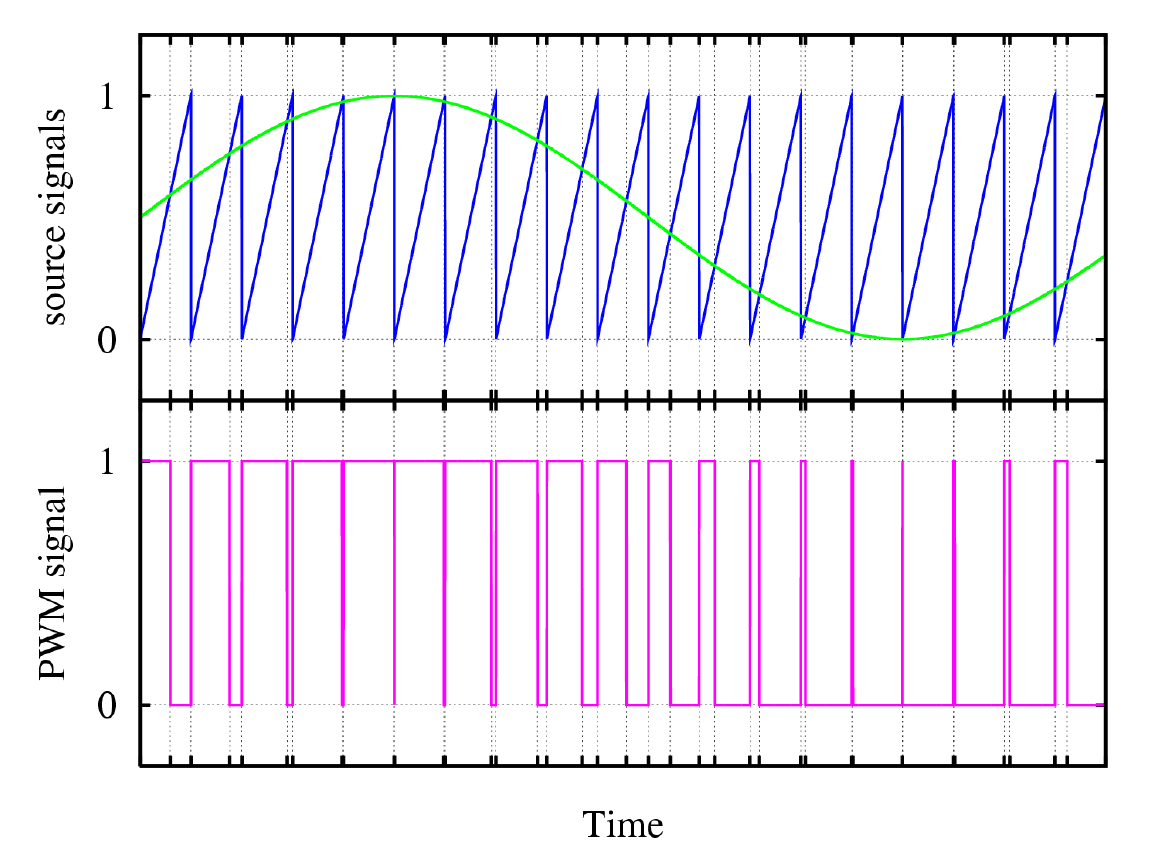
\includegraphics[width=\textwidth]{Bilder/BLDC_Aussteuerung.png}
% 	\captionof{figure}{Aussteuerung einer Phase, \cite{Vorlesung Aussteuerung}}
% 	\label{Aussteuerung}
% \end{Figure}

% \noindent
% Die Schematische Funktionsweise eines Brushless DC Motors sieht wie folgt aus. 
% Mittels 3 Halbbrücken werden die drei Phasen des Motors getrennt angesteuert und der Motor gesteuert, 
% beziehungsweise geregelt(vgl. Abbildung \ref*{Motor_Schematic}). 
% Die Geschwindigkeit wird vorgegeben, indem die Winkelgeschwindigkeit $ \omega $ eingestellt wird. 
%  $ \omega = 2\pi \cdot n = \frac{d\varphi}{dt} $   
%  \newline
% Die Spulenspannung wird durch $ u(t) = U \cdot sin(\omega \cdot t + \varphi_U) $ eingestellt. 
% \begin{Figure}
% 	% \resizebox{0.1\columnwidth}{!} 
% 	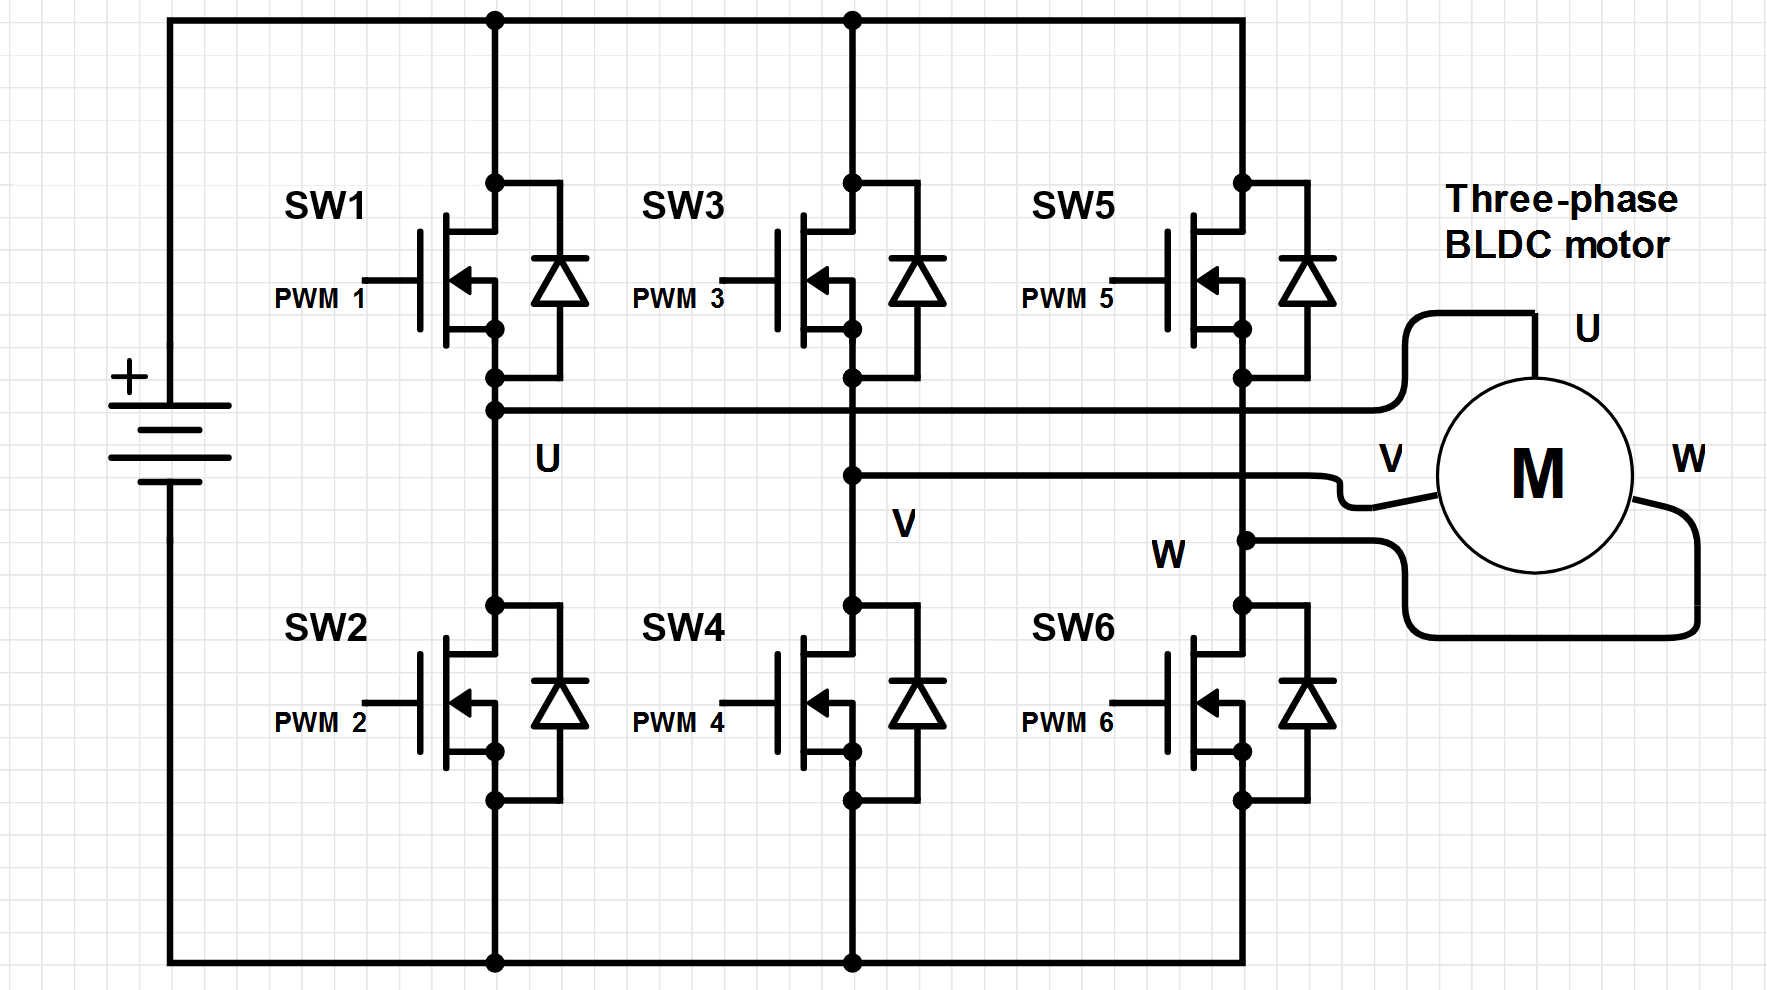
\includegraphics[width=\textwidth]{Bilder/BLDC_Schematic.png}
% 	\captionof{figure}{Schematische Funktionsweise eines BLDC Motors \cite{Motor_Ansteuerung}}
% 	\label{Motor_Schematic}
% \end{Figure}

% \subsubsection{Folgerung}
% Da sich der eingestellte Strom sehr schnell verändert und das Thermische System langsamer ist als die Motoransteuerung, 
% kann davon ausgegangen werden, dass in den Leitungen ein konstanter Strom fließt. 
% Es wird angenommen dass bei maximalem Drehmoment ein Strangstrom von bis zu $I_{Strang} = 5 A $  fließt. 

\section{Thermisches Design}
Industriestandards empfehlen Leiterbahnquerschnitte abhängig von der Strombelastung \cite{ipc}.
\newline
\subsection{Platinenaufbau}
Der Aufbau einer 2 lagigen Platine ist in Abbildung \ref*{pcb_im} dargestellt. 
\newline
Die mittlere Schicht der Platine besteht aus FR4, einem $ 1,5mm $ breiten Dielektrikum \cite{PCB_Querschnitt}. 
Die Leiterbahnenhöhe auf Ober- und Unterseite betragen jeweils $ 35 \mu m$ \cite{aisler}.
\begin{Figure}
	% \resizebox{0.1\columnwidth}{!} 
	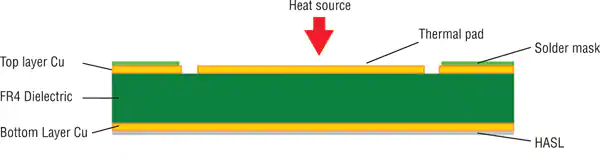
\includegraphics[width=\textwidth]{Bilder/PCB_Querschnitt.png}
	\captionof{figure}{Querschnitt einer  Platine \cite{PCB_Querschnitt}}
	\label{pcb_im}
\end{Figure}

\noindent
Durch Vias kann die Wärmeenergie schneller durch die Platine fließen. 
Dieser Fall wird nicht untersucht.
% Die Wärme fließt durch das Dielektrikum und auch über die Luft. 

\noindent



\subsection{Überprüfung des Vorgabewerts}
Die Arbeit widmet sich der Bestimmung des Thermischen Widerstands und der 
Platinenerwärmung durch den eingestellten Strom. 
\newline
% Für einen Strom von $I_{Strang} = 5 A $ und einer maximalen Erwärmung von $10 K$ ergibt sich nach dem Industriestandard eine
% Leiterbahnbreite von $b = 4 mm $ \cite{ipc}. 
Für die Arbeit wird die Platine für einen Strom von $I_{Strang} = 5 A $ ausgelegt. 
\newline
Nach Industriestandard ist für eine maximale Erwärmung von $10 K$ eine Leiterbahnbreite von $b = 4 mm $ notwendig\cite{ipc}. 
% und eine Leiterbahnbreite von $b = 4 mm $ untersucht.
Die Platine hat die Maße $15mm x 25mm$
Die Abmaße der zu simulierende Platine sind in Abbildung \ref*{geometry} ersichtlich.


\begin{Figure}
	% \resizebox{0.1\columnwidth}{!} 
	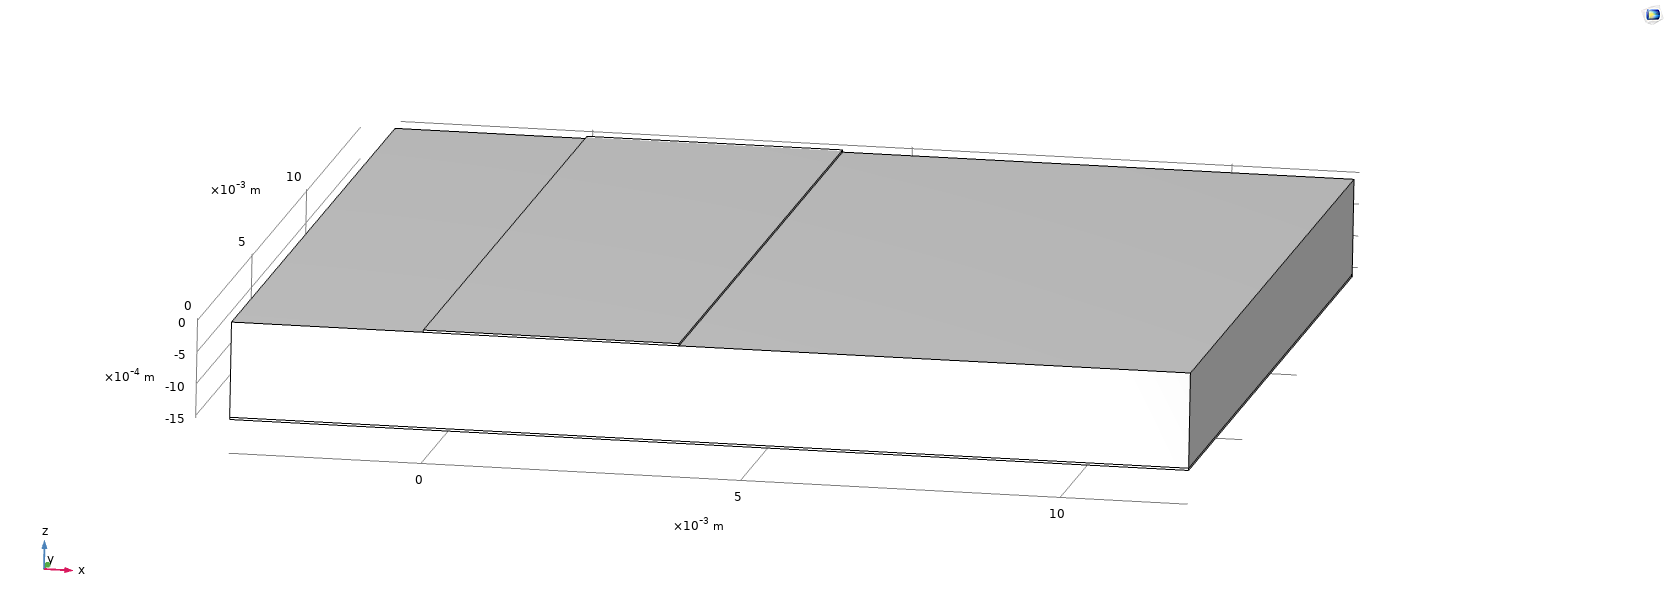
\includegraphics[width=\textwidth]{Bilder/Geometrie.png}
	\captionof{figure}{Geometrie der verwendeten Platine}
	\label{geometry}
\end{Figure}


\section{Händische Rechnung}
\subsection{Vorbedinungen}
Der Wärmestrom wird durch den elektrischen Strom der Leiterbahn und den Widerstand des Leiters bestimmt. 
\newline
Die elektrische Leitfähigkeit von Kupfer betragt 
\newline
$ \rho_{Cu} = \frac{58.1\cdot 10^6}{S \cdot m^{-1}} $ \cite{Waermefluss}.
\newline
Die zu simmulierende Leiterbahnlänge betragt
\newline
 $l = 15 mm$.
\newline
Die Querschnittsfläche der Leiterbahn betragt: 
\begin{equation}
	A = b \cdot h = 4 mm \cdot 35 \mu m = 140 \cdot 10 ^{-9} m^2
\end{equation}
Der Widerstand der Leiterbahn betragt: 
\begin{equation}
	R_{Leiter} = \frac{1}{\rho} \cdot \frac{l}{A} = 1,84 \cdot 10^{-3} \Omega
\end{equation}
\noindent
Der elektrische Schaltplan ist in Abbildung \ref*{Schaltplan} ersichtlich.  \newline
Es stellt sich eine Spannung über den Widerstand ein, vgl. Formel \ref*{Spannung}. 
\begin{equation}
	U_{Verlust} =  I_{Strang} \cdot R_{Leiter}
	\label{Spannung}
\end{equation}
\noindent
Die Verlustspannung betragt $U_{Verlust} = 5A \cdot 1,84 \cdot 10^{-3} \Omega = 9.2 mV$. 
Die elektrische Verlustleistung wird mit Formel \ref*{Leistung_Strom} berechnet: 
Es wird
$ P_{Thermisch} = (5A)^2 \cdot 1,84 \cdot 10^{-3} \Omega = 46 \cdot 10^{-3} W $ 
in das System eingeprägt.
Die Erwärmung wird mit Formel \ref*{Erwaermung} berechnet.
\begin{equation}
	\Delta T = P_{Thermisch} \cdot \Theta_{Junction, Ambient}
	\label{Erwaermung}
\end{equation}

\subsection{Berechnung }

\noindent
Die Berechnung der Erwärmung erfolgt mit dem thermischen Widerständen $\Theta$, vgl Formel \ref*{therm_Widerstand}.
\begin{equation}
	\Theta_{Junction, Ambient} = \frac{\frac{1}{h}}{A}
	\label{therm_Widerstand}
\end{equation}
Der Wärme-Transfer-Koeffizient zwischen Platine und Umgebung 
wird mit $ h = 10 \frac{W}{m^2K}$ angenommen \cite{TI_Thermal} .\newline
%  Es wird ein Ersatzschaltbild entworfen. 
Der thermische Widerstand $\Theta_{Junction, Ambient}$  wird nach Formel \ref*{formel} berechnet . 
\newline
Für den Wärmestrom wird die gesamte Oberfläche der Platine verwendet. 
Die Fläche der Oberseite und der Unterseite der Platine betragen: \newline
$A = 2\cdot 15mm \cdot 25mm$. 

\begin{equation}
	\Theta_{Junction, Ambient} = \frac{\frac{1}{10 \frac{W}{m^2K}}}{ 2\cdot 15mm \cdot 25mm} = 133 \frac{K}{W}
	\label{formel}
\end{equation}
Die Platine erwärmt sich nach der Formel \ref{Erwaermung} um \newline
$\Delta T = 46 \cdot 10^{-3} W \cdot 133 \frac{K }{W} = 6,1 K  $.

\subsection{Elektrischer Schaltplan für den Wärmestrom }
Um den Wert genauer zu bestimmen wird ein Ersatzschaltbild erstellt.
Es werden die thermischen Widerstände berechnet. 
Das Ersatzschaltbild wird ohne thermische Kapazitäten dargestellt, da uns der statische Zustand interessiert, nicht der transiente.
Um das System noch von Hand zu simmulieren, wird angenommen, dass der Wärmestrom nur nach oben und nach unten fließt. 
Der thermische Widerstand wird durch Formel \ref*{thermischerWiderstand} berechnet. 
\begin{equation}
	\Theta =  \frac{Höhe}{A \cdot \lambda}
	\label{thermischerWiderstand}
\end{equation}
\newline \noindent
Die thermische Leitfähigkeit von Kupfer beträgt:  \newline 
$\lambda_{Cu} = 360 \frac{W}{m K}$  \cite{Waermefluss} \newline
Für den spezifischen Fall betragt der thermische Widerstand von der Leiterbahn:  \newline
$\Theta_{Leiterbahn} = \frac{35 \mu m}{4mm \cdot 15mm \cdot 360 \frac{W}{m\cdot K}} = 1,62\cdot 10^{-3} \frac{K}{W}$
\newline \noindent
Die thermische Leitfähigkeit von FR4 beträgt: 
\newline
 $\lambda_{FR4} = 0,3 \frac{W}{m K}$ \cite{Waermefluss} \newline
Für den spezifischen Fall betragt der thermische Widerstand von dem Dielektrikum: 
\newline
$\Theta_{FR4} = \frac{1,5 mm}{4mm \cdot 15mm \cdot 0,3 \frac{W}{m\cdot K}} = 83,3 \frac{K}{W}$
\newline
Der thermische Widerstand zwischen Leiterbahn und Ambient beträgt: 
\newline
$\Theta_{Leiterbahn, Ambient} =  \frac{\frac{1}{10 \frac{W}{m^2K}}}{  4mm \cdot 15mm} = 1666 \frac{K}{W} $
\newline
Der thermische Widerstand zwischen Platine ohne Leiterbahn und Ambient beträgt: 
\newline
$\Theta_{PCB, Ambient} = \frac{\frac{1}{10 \frac{W}{m^2K}}}{ 2\cdot 25mm \cdot 15mm - 4mm \cdot 15mm} = 134 \frac{K}{W} $
% \frac{\frac{1}{10 \frac{W}{m^2K}}}{  4mm \cdot 15mm} = 1666 \frac{K}{W} $
\newline
Es wird eine Parallelschaltung entwickelt. 
\newline
Ein Teil des Wärmestroms fließt über die Leiterbahn direkt an die Umgebung. 
\newline
Ein anderer Teil fließt senkrecht durch die Platine und gibt dort die Wärmeenergie ab. 
Der Schaltplan ist in Abbildung \ref*{Schaltplan} dargestellt. 
\begin{Figure}
	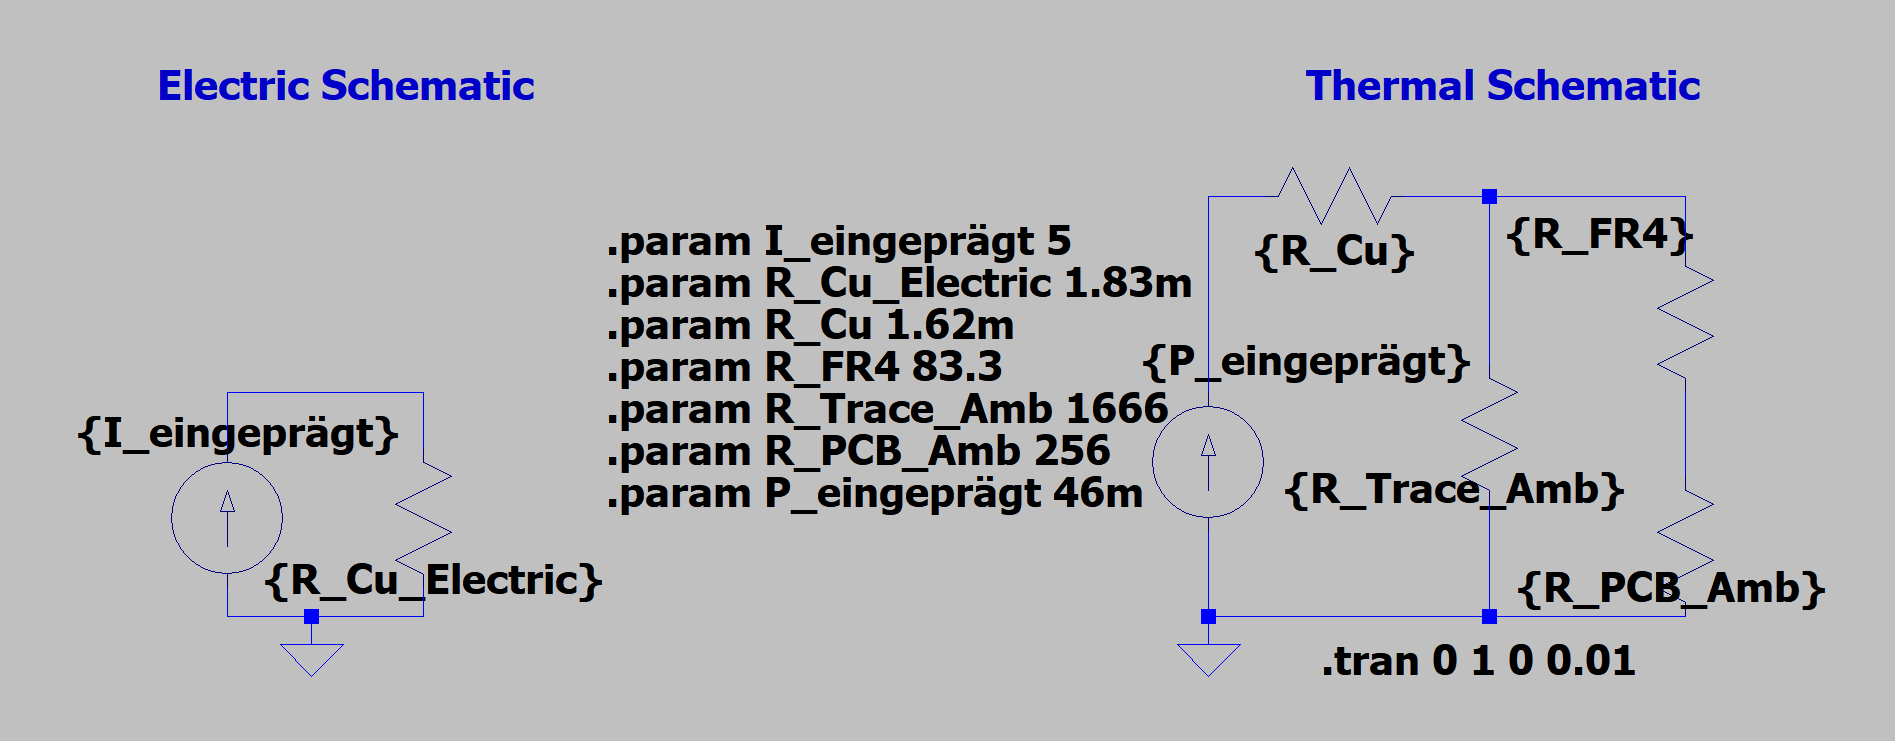
\includegraphics[width=\textwidth]{Bilder/Schaltplan.png}
	\captionof{figure}{Schaltplan: Elektrischer Stromkreis (links) 
	Schaltplan: Statische Temperatur (rechts)}
	\label{Schaltplan}
\end{Figure}
\noindent
Die Leistung in Abbildung \ref{Schaltplan} stellt die Stromquelle dar. 
Die Spannung ist die Temperaturerhöhung zur Referenztemperatur. 
Die Widerstände sind die thermischen Widerstände zwischen den Elementen. 
\newline
Laut Spice Model erwärmt sich die Platine um $\Delta T = 8,8K$


\section{Simulation}
Die berechneten Werte werden in Comsol überprüft.
\subsection{Allgemein}
An einem Ende wird Strom eingeprägt. Am anderen Ende ist Masse.
Die Geometrie ist in Abbildung \ref*{geometry} ersichtlich.
\newline
% \noindent
% Mit Formel \ref*{Super_Elektro} berechnet das Simulationsprogramm die Elektrotechnik.
% \begin{equation}
% 	\int_{\alpha \Omega}^{} J \cdot n\,dS\ = I_O 
% 	\label{Super_Elektro}
% \end{equation}
% \noindent
% Mit Formel \ref*{Super_Insulation} berechnet das Simulationsprogramm die Wärmeisolierung.
% \begin{equation}
% -n \cdot q = 0
% \label{Super_Insulation}
% \end{equation}
% \noindent
Mit Formel \ref*{Super_SurfacetoAmb} berechnet das Simulationsprogramm den Wärmefluss an die Umwelt.
\begin{equation}
	-n \cdot q = \epsilon \sigma (T^4_{amb} - T^4)
	\label{Super_SurfacetoAmb}
	\end{equation}
	\noindent
	Mit Formel \ref*{Super_Multi1} und \ref*{Super_Multi2} berechnet das Simulationsprogramm das Zusammenspiel der Elektrotechnik un der Thermodynamik.

	\begin{equation}
		\rho c_p u \cdot \nabla = \nabla \cdot (\kappa \nabla T)+ Q_e
		\label{Super_Multi1}
		\end{equation}

		\begin{equation}
			Q_e = J \cdot E
			\label{Super_Multi2}
			\end{equation}



\subsection{Netz}
Die Vernetzung ist in Abbildung \ref*{net} dargestellt.
Die Breiten der beiden Geometrien unterscheiden sich deutlich. 
\newline
Ein Abmaß beträgt $ 15mm $. Das andere Abmaß ist $ 35 \mu m$.  
\newline
Wird das Netz gröber als normal eingestellt werden folgende Warnungen erzeugt: 
\begin{quote}
Edge is much shorter than the specified minimum element size.
\newline
Face is (or has a narrow region that is) much smaller than the specified minimum element size.
\newline
Domain has a region that is much thinner than the specified minimum element size.
\end{quote}
\noindent
Das Netz muss genauer eingstellt werden damit dieser Fehler nicht mehr auftritt. 
\newline
Es kann nur eine endliche Fläche untersucht werden.
Die Simulationszeiten verlängern sich bei und großen Flächen stark.
\newline
Unabhängig ob Warnungen beim Vernetzen auftreten unterscheiden sich die Ergebnisse der berechneten Spannung und der Temperatur nicht.
\newline
Die Netzunabhängigkeit wurde überprüft und ist gegeben. 

\begin{Figure}
	% \resizebox{0.1\columnwidth}{!} 
	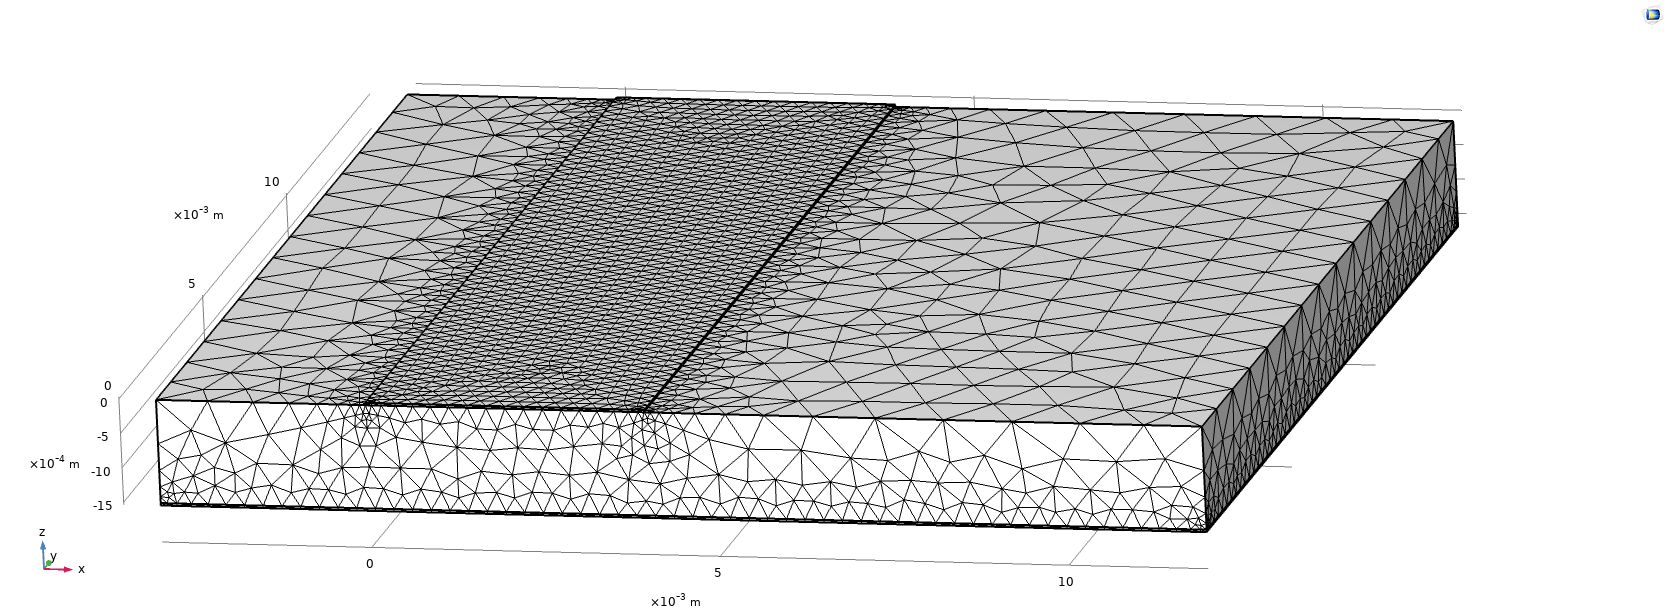
\includegraphics[width=\textwidth]{Bilder/net.png}
	\captionof{figure}{Vernetzung des Models}
	\label{net}
\end{Figure}

\subsection{Spannungsverlauf}
Die Spannung verlauft linear über die Leiterbahn. 
Das stimmt mit dem erwartenden Ergebnis überein. 
Die maximale Spannung betragt $ U_{Verlust} = 9,22mV$, vgl. Abbildung \ref{voltage}.

\begin{Figure}
	% \resizebox{0.1\columnwidth}{!} 
	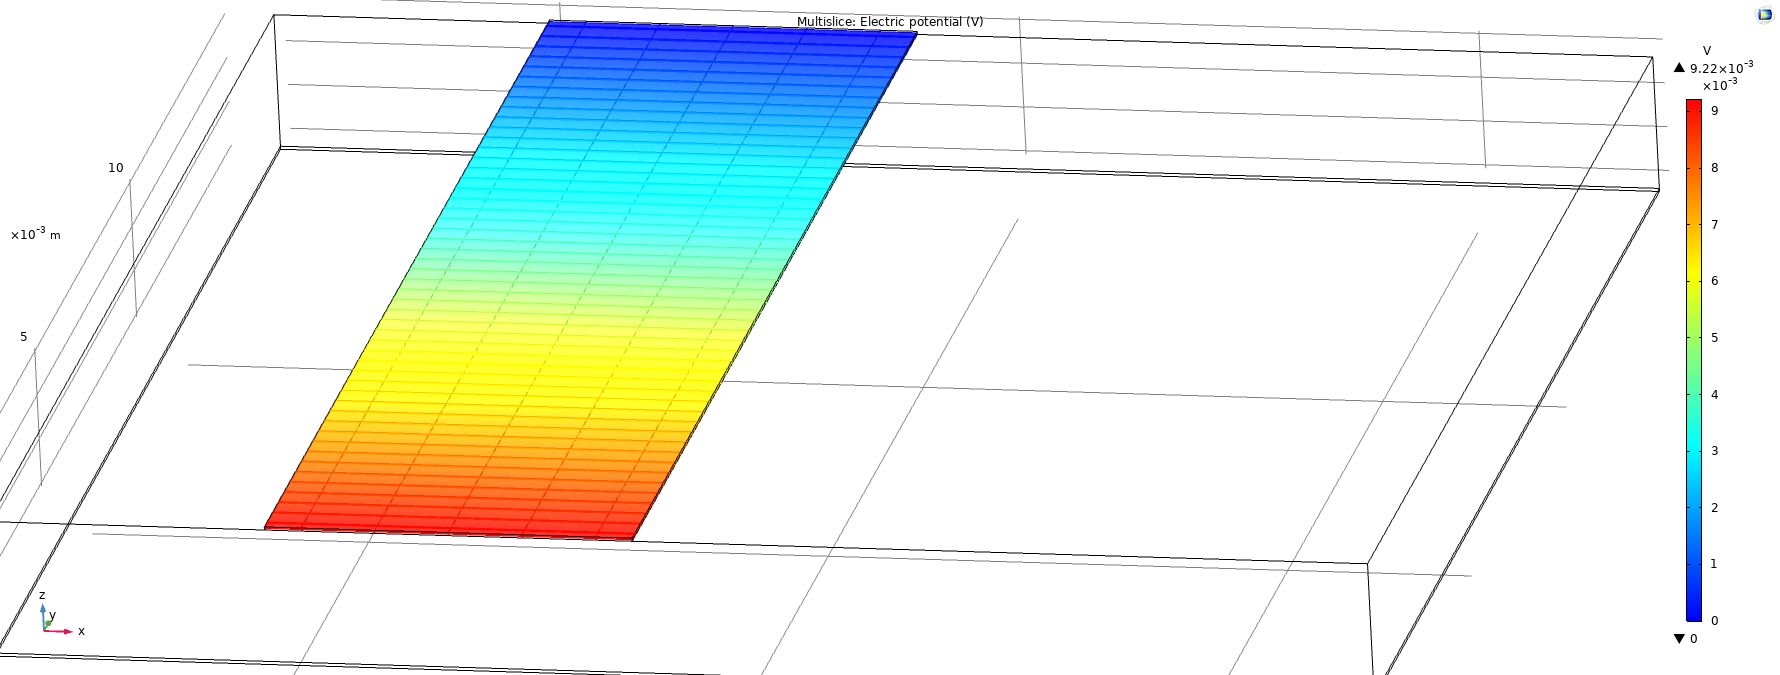
\includegraphics[width=\textwidth]{Bilder/voltage.png}
	\captionof{figure}{Spannungsabfall über der Leiterbahn}
	\label{voltage}
\end{Figure}

\subsection{Statischer Temperaturverlauf}

\begin{Figure}
	% \resizebox{0.1\columnwidth}{!} 
	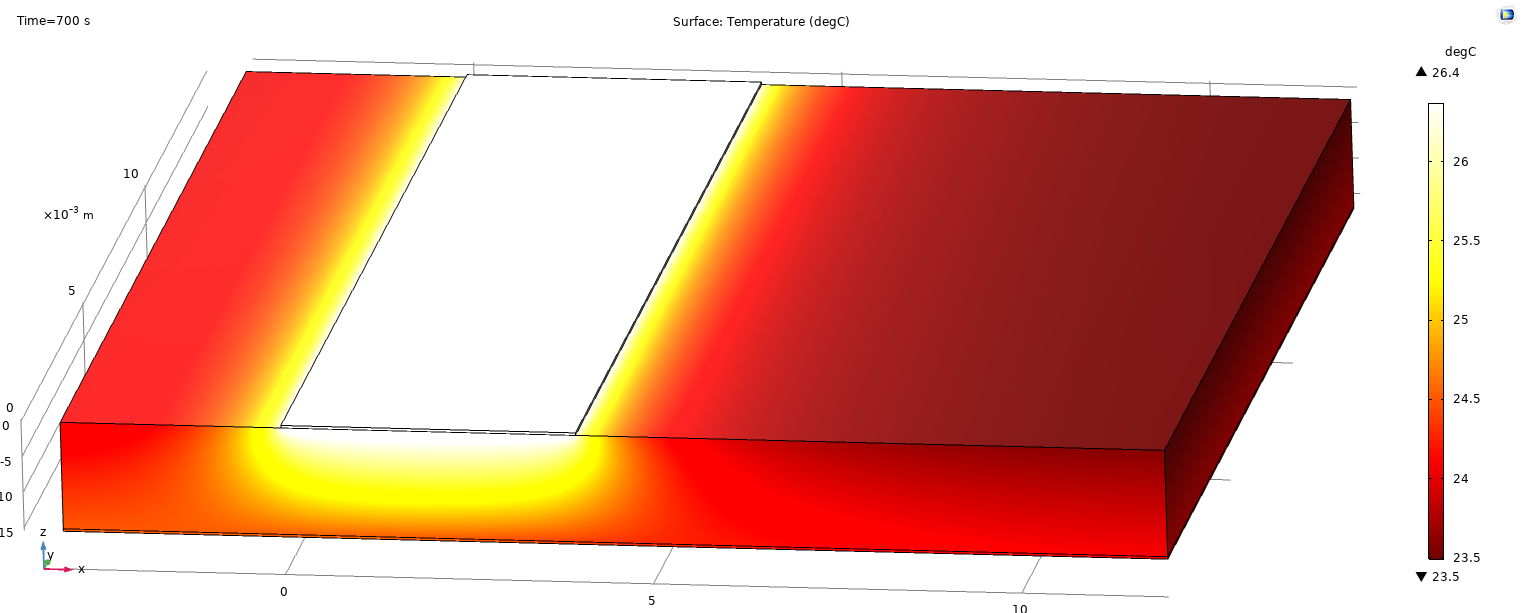
\includegraphics[width=\textwidth]{Bilder/Thermal_static.png}
	\captionof{figure}{Thermische Endzustände}
	\label{static_thermal}
\end{Figure}
\noindent
Die Temperatur erhöht sich in der Simulation in der Mitte der Leiterbahn um $6,4 K$.
Kupfer ist ein sehr guter Wärmeleiter. Er hat einen sehr geringer Widerstand. 
\newline
Am Rand der Leiterbahn ist die Temperatur immernoch nahezu identisch. Die Wärme verteilt sich sehr gut. 
Das Dielektrikum hingegen hat einen großen thermischen Widerstand. 
Die Unterseite der Platine ist bereits $2K$ kälter., vgl. Abbildung \ref{static_thermal}. 
\newline
Bereits wenige Millimeter daneben ist die Temperatur deutlich niedriger, vgl. Abbildung \ref{schnitt}.
$8 mm$ neben der Leiterbahn steigt die Oberflächentemperatur um $3K$
\begin{Figure}
	% \resizebox{0.1\columnwidth}{!} 
	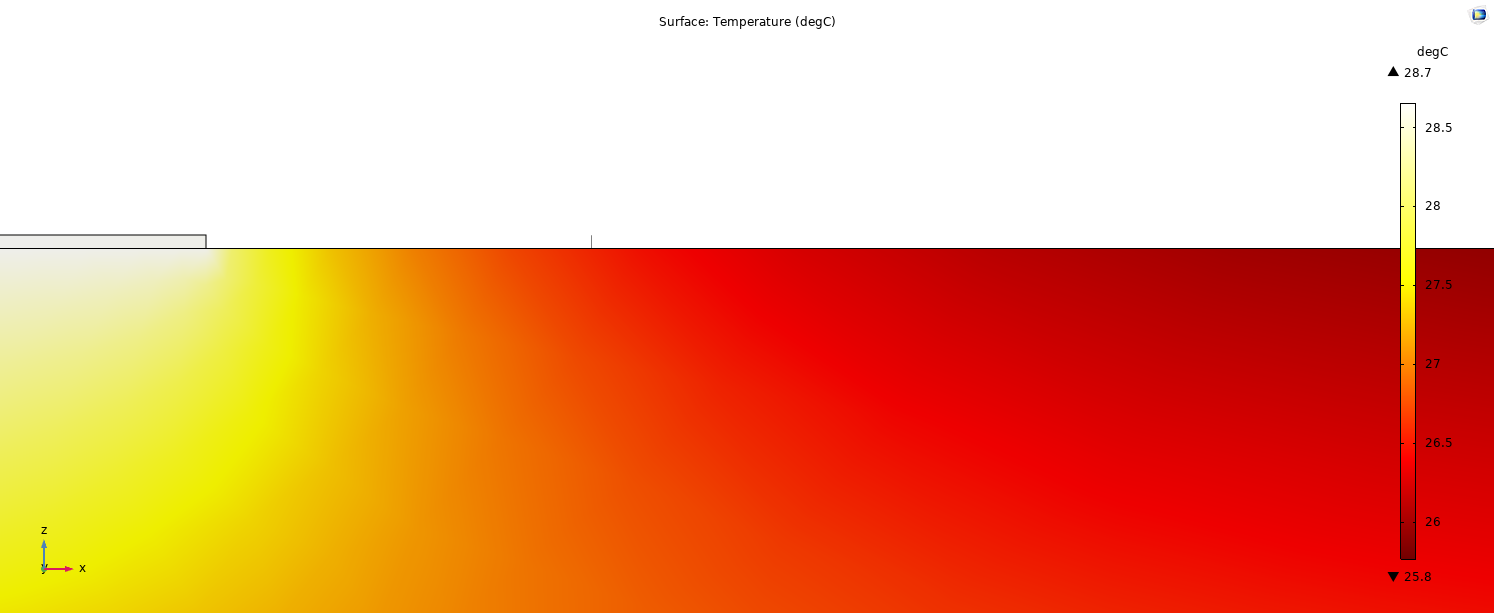
\includegraphics[width=\textwidth]{Bilder/schnitt.png}
	\captionof{figure}{Detailansicht Wärmefluss auf der Platine}
	\label{schnitt}
\end{Figure}

\subsection{Transienter Temperaturverlauf}
In Abbildung \ref{timedep} ist der transiente Verlauf für einen Punkt im Mittelpunkt der Leiterbahn 
$8 mm$ neben der Leiterbahn dargestellt.

\begin{Figure}
	% \resizebox{0.1\columnwidth}{!} 
	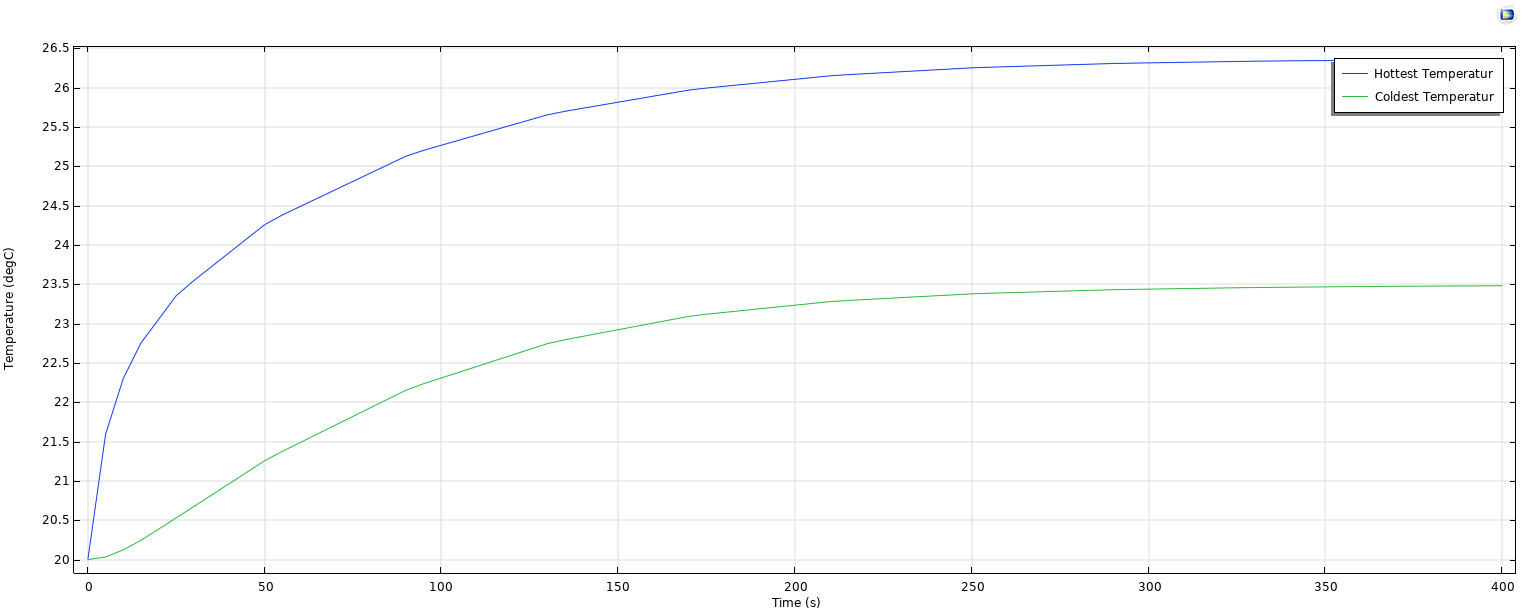
\includegraphics[width=\textwidth]{Bilder/time_dep.png}
	\captionof{figure}{Änderung der Temperatur mit der Zeit}
	\label{timedep}
\end{Figure}
\noindent
Die Simulation ist zeitabhängig für $ t < 350s $. 
Für Zeiten $ t > 350s $ ändert sich das Ergebnis nur noch minimal. 
Die statische Endtemperatur ist erreicht. 
Die Kurvenform ist die einer Differentialgleichen. $ T(t) = K \cdot e^{\lambda t} $ mit
$ \lambda  < 0$. Es ist ein stabiles System. 
Die eingeprägte Leistung ist gleich der abgegeben Leistung. 
Wegen der Trägheit des Systems ist auf den schematischen Schaltplan in Abbildung \ref{trans_thermal} zu schließen. 
Das Einschwingverhalten von der grünen Bahn lässt auf in Reihe geschaltete $PT_1$ Glieder schließen. 
\begin{Figure}
	% \resizebox{0.1\columnwidth}{!} 
	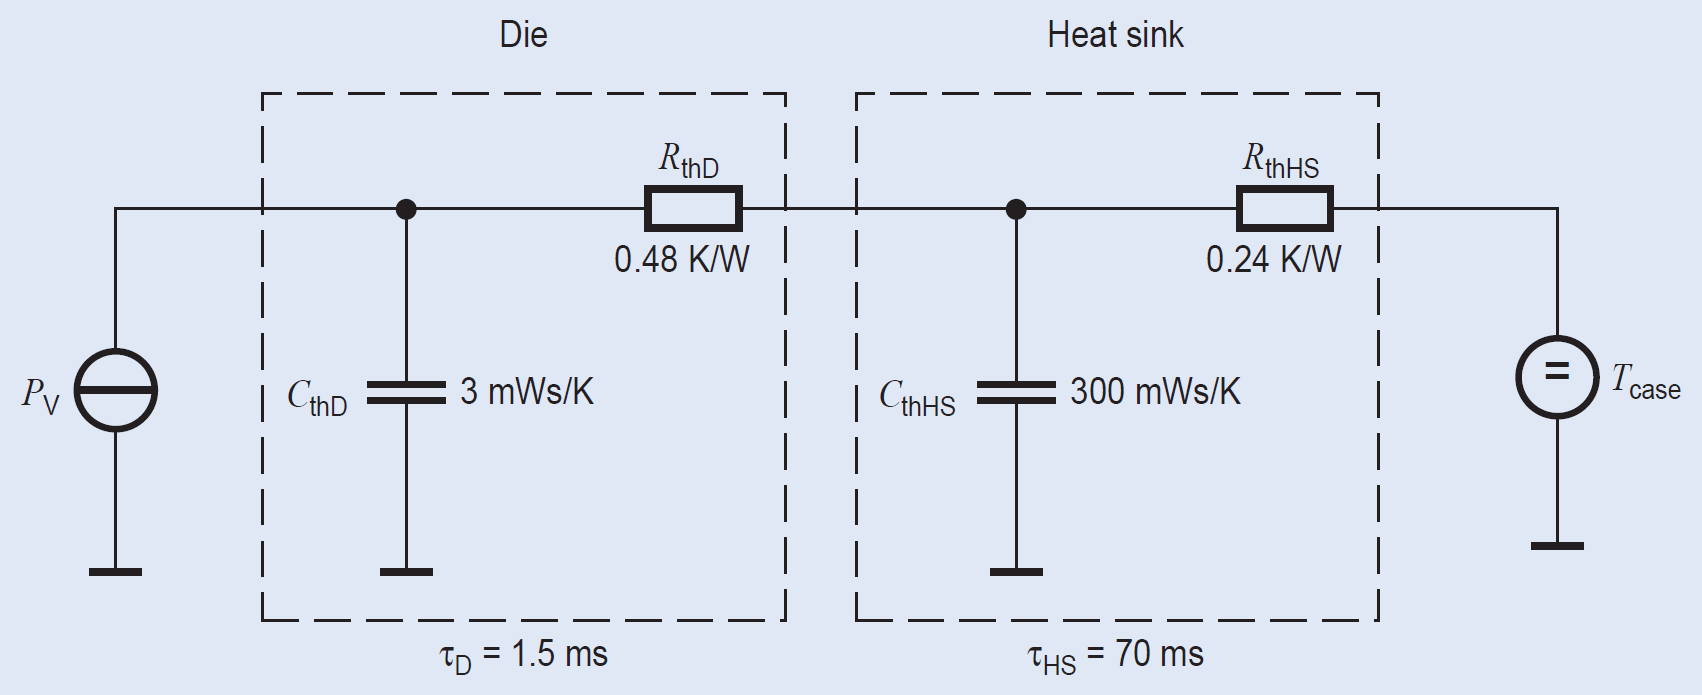
\includegraphics[width=\textwidth]{Bilder/trans_thermal.png}
	\captionof{figure}{Ersatzschaltplan: Thermodynamsiches Verhalten \cite{infineon}}
	\label{trans_thermal}
\end{Figure}

\section{Fazit}
Der Leiterbahnquerschnitt wurde nach geltendem Industriestandard ermittelt. 
\newline
Die erste Formel gilt als Daumenregel und ist von der simulierten Lösung um $\Delta T = 6,1K - 6,4K = 0,3K$ entfernt. \newline
Das $h $ in Formel \ref*{Erwaermung} bezieht sich auf eine 2-Fach so große Fläche als simmuliert wurde. Daher weicht der Wert ab. \newline
Die Spice Simulation mit $\Delta T = 8,8K - 6,4K = 2,4 K$ ist weiter entfernt.  \newline
Es wurde davon ausgegangen, dass der Wärmestrom der nicht direkt an die Umwelt abgegeben wird
immer 1,5mm durch das Dielektrikum fließt. Die Annahme scheint nicht zu stimmen. \newline
$ \Theta_{*, Ambient} $ sind die dominierenden Faktoren in der Gleichung.  \newline
Auch die FEM-Simulation hat einen Fehler in der Praxis. 
Die Platinen in der Industrie sind größer als die simulierte Platine.
Mit den berechneten Werten von Comsol kann mit Grundlagen der Regelungstechnik ein genaueres Spice Model erzeugt werden.  \newline
Die Formeln aus der Industrie enthalten Sicherheiten.
\newline
Für die meisten Platinenlayouts sind die Werte aus der Industrie in Ordnung und der Fehler vernachlässigbar. 
\newline
Wegen fehlender aktiver Last konnten keine Messwerte aufgenommen werden.
%  bei guter Auslegung der Platine. 
\noindent
\begin{thebibliography}{9}

\bibitem{Waermefluss}
Wuerth Elektronik eiSos  [online], [Zugriff am 22.12.2021] Verfuegbar unter:
 https://www.we-online.com/web/en/index.php/show/media/04
 \_leiterplatte/2011\_2/ relaunch/produkte\-5/heatsink/neu\_2011/
 TecReport\-01\-2011\-EN-S.pdf

\bibitem{Vorlesung Aussteuerung}
Prof. Dr. Reddig, Vorlesung Leistungselektronik

\bibitem{Elko}
TDK-Lambda Germany GmbH [online], [Zugriff am 22.12.2021] Verfuegbar unter:	https://www.emea.lambda.tdk.com/de/KB/Was-Sie-über-die-Lebensdauer-von-Stromversorgungen-wissen-sollten.pdf
Aachen, TDK-Lambda Germany GmbH



\bibitem{TI_Thermal}
Texas Instruments, 01.04.2013, Zugriff am 22.12.2021] Verfuegbar unter: https://www.ti.com/lit/pdf/snva419?keyMatch=
THERMAL\%20DESIGN\%20BY\%20INSIGHT\%20NOT\%
20HINDSIGHT

\bibitem{ipc}
IPC  [online], [Zugriff am 22.12.2021] Verfuegbar unter https://www.ipc.org/TOC/IPC-2221.pdf, United States, IPC

\bibitem{PCB_Querschnitt}
Cree, Inc. Optimizing PCB Thermal Performance for Cree XLamp LEDs 22.12.2010, [Zugriff am 22.12.2021] Verfuegbar unter https://www.digikey.de/en/articles/optimizing-pcb-thermal-performance-for-cree-xlamp-leds

\bibitem{aisler}
Aisler B. V.  [online], [Zugriff am 22.12.2021] Verfuegbar unter https://aisler.net/help/design-rules-and-specifications/specifications

\bibitem{infineon}
Infineon Technologies AG, 11.07.2000, Zugriff am 22.12.2021] Verfuegbar unter: https://www.infineon.com/dgdl/smdpack.pdf?fileId=
db3a304330f6860601311905ea1d4599


\end{thebibliography}

\end{multicols}
 

\end{document}
